\begin{example}
  \label{ex_contrib_variant}
  The rewriting rule illustrated below modifies a rule from~\cite[Example 6]{plump2018modular} by removing all interface edges and adding a node with identifier $5$ and three self-loops labeled $0$.
  \begin{center}
      \resizebox{0.6\textwidth}{!}{
          \begin{tikzpicture}
              \graphbox{$L$}{0mm}{0mm}{35mm}{35mm}{2mm}{-5mm}{
                  \coordinate (delta) at (0,-18mm);
                  \node[draw,circle] (l1) at ($(delta) + (-1,1.5)$) {1};
                  \node[draw,circle] (l2) at ($(delta) + (1,1.5)$) {2};
                  \node[draw,circle] (l3) at ($(delta) + (0,0)$) {3};
                  \draw[->] (l1) -- (l3) node[midway,left] {s};
                  \draw[->] (l2) -- (l3) node[midway,right] {s};
                  \draw[->] (l3) edge [loop below] node {0} (l3);
              }
              \graphbox{$K$}{40mm}{0mm}{35mm}{35mm}{2mm}{-5mm}{
                  \coordinate (delta) at (0,-18mm);
                  \coordinate (interfaceorigin) at ($(delta) +(5,0)$);
                  \node[draw,circle] (r1) at ($(delta) +(-1,1.5)$) {1};
                  \node[draw,circle] (r2) at ($(delta) +(0.5,1.5)$) {2};
                  \node[draw,circle] (r3) at ($(delta) + (0,0)$) {3};
              }
              \graphbox{$R$}{80mm}{0mm}{50mm}{35mm}{2mm}{-5mm}{
                  \coordinate (delta) at (-10mm,-18mm);
                  \node[draw,circle] (r1) at ($(delta) + (-1,1.5)$) {1};
                  \node[draw,circle] (r2) at ($(delta) + (0.5,1.5)$) {2};
                  \node[draw,circle] (r3) at ($(delta) + (0,0)$) {3};
                  \node[draw,circle] (r4) at ($(delta) + (1,0)$) {4};
                  \draw[->] (r1) -- (r3) node[midway,left] {s};
                  \draw[->] (r2) -- (r4) node[midway,right] {s};
                  \draw[->] (r4) edge [loop below] node {0} (r4);
                  \draw[->] (r3) edge [loop below] node {0} (r3);
                  \node[draw,circle] (r5) at ($(r2) + (1.5,0)$) {5};
                  \draw[->] (r5) edge [loop below] node {0} (r5);
                  \draw[->] (r5) edge [loop right] node {0} (r5);
                  \draw[->] (r5) edge [loop left] node {0} (r5);
              }
              \node () at (38mm,-18mm) {$\leftarrowtail$};
              \node () at (77mm,-18mm) {$\rightarrowtail$};
          \end{tikzpicture}
          }
  \end{center}
 
      Consider the ruler-graph $\mathcal{X} = (X)$ where $X$ is the graph
      \tikz[baseline=-0.5ex]{ 
              \node (x) at (0,0) {$\bullet$}; 
              \node (y) at (1,0) {$\bullet$};
              \node (z) at (2,0) {$\bullet$};
              \draw[->] (x) -- (y) node[midway, above] {$s$};
              \draw[->] (z) -- (y) node[midway, above] {$s$};
      } and there is no forbidden contexts. $\mathcal{X}$ has weight $1$ and $\mathbb{X} = \{X\}$.
      The set \( D(R,X) \) contains a unique element $R'$:
      \raisebox{2pt}{
          \scalebox{0.7}{\tikz[baseline=-0.5ex]{
          \node [draw,circle] (x) at (0,0) {1};
          \node[draw,circle] (y) at (1,0) {3};
          \draw[->] (x) -- (y) node[midway, above] {$s$};
      }}}. The rule is $X$-non-increasing under the function mapping the unique subgraph in $R$ to the same subgraph in $L$. 
    %   Since $F_X = \emptyset$, the number of $X$-occurrences not included in any occurrences of forbidden context in any rewriting step is predictable.
      By~\autoref{thm:termination_grs}, the rule terminates because \(|Mono(X,L)| - |Mono(X,R)| = 1 - 0 = 1 > 0 \). 
\end{example}
\begin{example}
  \label{ex:grs_aca}
  Consider the following rule $\rho$ from~\cite[Example 1]{bruggink2014termination}:
  \begin{center} 
  \resizebox{0.7\textwidth}{!}{
  \begin{tikzpicture}
      \graphbox{$L$}{0mm}{0mm}{34mm}{20mm}{2mm}{-5mm}{
          \coordinate (o) at (0mm,-3mm); 
          \node[draw,circle] (l1) at ($(o)+(-10mm,0mm)$) {1};
          \node[draw,circle] (l2) at ($(l1)+(2,0)$) {2};
          \node[draw,circle] (l3) at ($(l1) + (1,0)$) {3};
          \draw[->] (l1) -- (l3) node[midway,above] {a};
          \draw[->] (l3) -- (l2) node[midway,above] {a};
      }     
      \graphbox{$K$}{40mm}{0mm}{24mm}{20mm}{2mm}{-5mm}{
          \coordinate (o) at (5mm,-3mm); 
          \node[draw,circle] (l1) at ($(o)+(-10mm,0mm)$) {1};
          \node[draw,circle] (l2) at ($(l1)+(1,0)$) {2};
          % \node[draw,circle] (l3) at ($(l1) + (1,0)$) {$\ $};
          % \draw[->] (l1) -- (l3) node[midway,above] {a};
          % \draw[->] (l3) -- (l2) node[midway,above] {a};
      }    
      \graphbox{$R$}{70mm}{0mm}{45mm}{20mm}{2mm}{-5mm}{
        \coordinate (o) at (0mm,-3mm); 
        \node[draw,circle] (l1) at ($(o)+(-10mm,0mm)$) {1};
        \node[draw,circle] (l2) at ($(l1)+(2,0)$) {2};
        \node[draw,circle] (l3) at ($(l1) + (1,0)$) {3};
        \draw[->] (l1) -- (l3) node[midway,above] {a};
        \draw[->] (l3) -- (l2) node[midway,above] {a};
        \draw[->] (l3) edge [loop below] node {$c$} (l3);
      }    

      \node () at (37mm,-10mm) {$\leftarrowtail$};
      \node () at (67mm,-10mm) {$\rightarrowtail$};

      % \draw[>->] (51mm,2mm) -- (52mm,3mm);
  \end{tikzpicture}
  }
\end{center}
Consider the ruler-graph $\mathcal{X} = (L, f)$ where the underlying graph is $L$ and $f:L \rightarrowtail R$ is the inclusion function.
% The number of $L$-occurrences not included in any occurrences of the forbidden context $R$ in any rewriting step using this rule is predictable:
% the condition~\ref{hyp:inj_mono_x_l_to_r} is satisfied because $Mono(L,L)_F = \emptyset$; the condition~\ref{hyp:inj_mono_f_l_to_r} is satisfied because $Mono(R,L) = \emptyset$; the conditions~\ref{hyp:x_non_increasing} and~\ref{hyp:f_non_increasing} are satisfied under identity function; the condition~\ref{hyp:f_non_increasing} is satisfied because for the condition~\ref{hyp:f_non_increasing} we employ identity function. 
$\rho$ is $X$-non-increasing, and $\rho^{-1}$ is $X$-non-increasing and $F$-non-increasing. \todo{more details?}
Since we have additionally $\card{\operatorname{Mono}(X,L)_{\operatorname{NF}}} - 
\card{
    \Gamma(\operatorname{Mono}(\mathcal{X},L)_{\operatorname{NF}})
    }   -
\card{\operatorname{Mono}(X,R)_{\operatorname{NF}}} = 1 - 0 - 0 = 1 > 0$. The rule terminates by~\autoref{thm:termination_grs}.
\todo{check} 
\end{example} 
% Finally, we present a limitation of our approach.
\begin{example}
    \label{rem:d3:solution}  
    Our method can prove termination of the rewriting rule $\rho$ from~\cite[Example D.3]{endrullis2024generalized_arxiv_v2}:
    \begin{center}
        \resizebox{0.7\textwidth}{!}{
    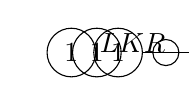
\begin{tikzpicture}  
       \graphbox{$L$}{0mm}{-11mm}{32mm}{15mm}{2mm}{-8mm}{  
           \node[draw,circle]  (x) at (-6mm,0mm) {1};  
           \node[draw,circle]  (y) at (6mm,0mm) {};  
         }  
         \graphbox{$K$}{33mm}{-11mm}{32mm}{15mm}{2mm}{-8mm}{  
           \node[draw,circle]  (x) at (-6mm,0mm) {1};  
         }  
         \graphbox{$R$}{66mm}{-11mm}{32mm}{15mm}{1mm}{-8mm}{  
          \node[draw,circle]  (x) at (-6mm,0mm) {1};  
          \node[draw,circle]  (y) at (6mm,0mm) {};  
          \draw[->]  (x) to (y);  
         }    
   \end{tikzpicture}
        }  
    \end{center}
    Let $\mathcal{X} = (L,f)$ be the ruler-graph where $f:L \rightarrowtail R$ is the unique interface preserving monomorphism from $L$ to $R$. 
    % The number of $X$-occurrences not included in any occurrences of the forbidden context $R$ in any $\rho$-rewriting step is predictable. 
    $\rho$ is $X$-non-increasing, and if $\mathcal{X}= (X,f:X \rightarrowtail F)$ then $\rho^{-1}$ is $X$-non-increasing and $F$-non-increasing. \todo{more details?}
    Since we have additionally $\card{\operatorname{Mono}(X,L)_{\operatorname{NF}}} - 
    \card{
        \Gamma(\operatorname{Mono}(\mathcal{X},L)_{\operatorname{NF}})
        } -
    \card{\operatorname{Mono}(X,R)_{\operatorname{NF}}}
    = 1 - 0 - 0 = 1 > 0$. The rule terminates by~\autoref{thm:termination_grs}.
  \end{example} 

% \begin{example}[Limitation]
%   The termination of the rewriting rule presented in~\cite[Ad-hoc routing protocol]{bruggink2014termination} cannot be proven by our method, because the property defined in~\autoref{def:predictable} is too restrictive.
% \end{example} 